\documentclass{article}
% Paquetes
\usepackage[utf8]{inputenc}
\usepackage[spanish]{babel}
\usepackage[]{amsthm}
\usepackage{amsmath}
\usepackage[]{amssymb}
\usepackage{graphicx}
\usepackage{wrapfig}
\usepackage[letterpaper, margin=1.5in]{geometry}
\usepackage[hidelinks]{hyperref}
\usepackage{csvsimple}
\usepackage{pdflscape}
\decimalpoint
\usepackage{float}
\usepackage{pdflscape}


\begin{document}
    \begin{titlepage}
        \begin{center}
            % School logo
            \begin{figure}
                \centering
                
\includegraphics[scale=0.13]{../../img/logo_itesm.png}\\ % Logo de la institución
            \end{figure}
            \vspace{5cm}
            % School data
            \LARGE{Instituto Tecnológico y de Estudios Superiores de Monterrey}\\
            \vspace{1cm}
            \large Escuela de Ingeniería y Ciencias \\
            \vspace{0.2cm}
            \large Ingeniería en Ciencias de Datos y Matemáticas \\
            \vspace{0.2cm}
            \large Análisis de Criptografía y Seguridad\\
            \vspace{1cm}
            \textbf{Actividad 4.3 Laboratorio 2 Attack Defense: Live Cracking WPA-PSK}\\ % Nombre de la tarea
            \vspace{0.7cm}
            % Tabla de integrantes del equipo
            \begin{table}[h!]
                \centering
                \begin{tabular}{ ||c|c|| }
                    \hline
                    Nombre & Matrícula \\
                    \hline
                    Julio Avelino Amador Fernández & A01276513 \\
                    \hline
                    Juan Pablo Echeagaray González & A00830646 \\
                    \hline
                    Verónica Victoria García De la Fuente & A00830383 \\
                    \hline
                    Erika Martínez Meneses & A01028621 \\
                    \hline
                    Emily Rebeca Méndez Cruz & A00830768 \\
                    \hline
                    Ana Paula Ruiz Alvaro & A01367467 \\
                    \hline
                \end{tabular}
            \end{table}
            \vspace{0.7cm}
            \large Dr. Alberto Francisco Martínez Herrera \\ % Nombre del profesor 1
            \vspace{0.2cm}
            \large Monterrey, Nuevo León \\
            \vspace{0.2cm}
            \large 11 de junio del 2022 \\
            \vspace{1cm}
        \end{center}
    \end{titlepage}
    
    
    Esta actividad consiste en la realización del laboratorio Live Cracking WPA-PSK del laboratorio de PENTEST, usando el Laboratorio virtual Attack-Defense, cuyo objetivo es descifrar el protocolo de enlace WPA para la red y obtener la frase de contraseña pre-compartida de la red \cite{farina}. La ventana inicial del laboratorio se ve como en la figura \ref{fig:wpa-before}.
    
    \section{Procedimiento}

        Como primer paso se verifica la lista de interfaces de red WiFi disponibles en la máquina a través del comando \texttt{iw dev} y como se observa en la figura \ref{fig:step2}, nos da como resultado una, la interfaz \texttt{wlan0}.
        
        Como siguiente paso para ver todas las redes presentes en las inmediaciones en 2.4 (b/g) banda Ghz se ejecutó airodump-ng en la interfaz \texttt{wlan0} y lo más importante que se nos muestra aquí (figura \ref{fig:step3}) es que SSID \texttt{HackMeIfYouCan} está operando en el canal 6. 
        
        Sabiendo esto, nos enfocamos en este canal que es el que nos interesa para vulnerar el \texttt{wlan0}, para lograr esto escribiremos los paquetes capturados en un archivo que llamamos \texttt{test}, esto se logra a través del comando \texttt{airodump-ng wlan0 -c 6 -w test}, en el resultado, el cual se muestra en la figura \ref{fig:step4}, podemos observar que hay un cliente conectado a la red.
        
        A continuación lo que necesitamos es un WPA 4-way handshake para lanzar un \emph{cracking attack} por lo que es necesario enviar \texttt{deauth packets} al cliente el cual está conectado a BSSID \texttt{A2:E9:68:D3:03:10} para desconectarlo y así cuando se vuelva a conectar al BSSID el protocolo de enlace sea capturado por airodump-ng. Para esto podemos abrir otro lab link y a través del comando \texttt{aireplay-ng | less} ver las opciones que tenemos. En \texttt{replay options} podemos encontrar el comando necesario para establecer la dirección MAC del punto de acceso y en attack modes encontramos el ataque que deseamos realizar. Nótese que pudimos haber esperado a que el usuario se desconectase y conectase por su cuenta de nuevo, pero para fines prácticos la aproximación que tomamos es más que suficiente.

        Al ejecutar el comando \texttt{aireplay-ng -0 100 -a A2:E9:68:D3:03:10 wlan0} como se muestra en la figura \ref{fig:step5} el cliente se desconecta y se vuelve a conectar al AP logrando que el handshake sea capturado por \texttt{airodump-ng}, esto lo podemos observar en la figura \ref{fig:step6}.
        
        A continuación salimos de \texttt{airodump-ng} y ejecutamos \texttt{aircrack-ng} en el archivo de paquete capturado mediante el comando \texttt{aircrack-ng -w 100-common-passwords.txt -0 test-0?.cap}. Y finalmente encontramos que a clave pre-compartida es \texttt{friendship}, este resultado se puede observar en la figura \ref{fig:step7}.

        Después de realizar este proceso la pantalla del reto se actualiza para informarnos que hemos conseguido la bandera, como se muestra en la figura \ref{fig:wpa-after}.

    \bibliographystyle{apalike}
    \bibliography{references.bib}

    \clearpage
    \appendix
    \section{Evidencias}
    
        \begin{landscape}
            \begin{figure}[!h]
                \centering
                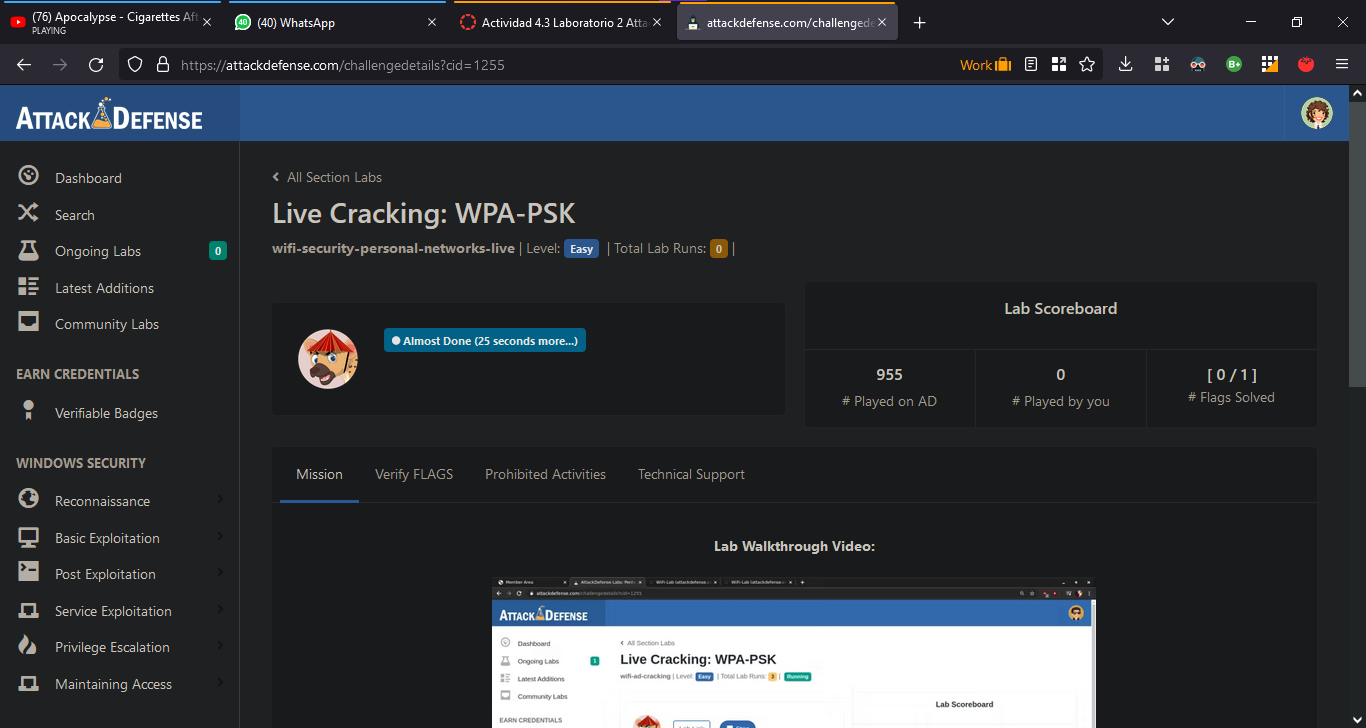
\includegraphics[scale=0.5]{img/wpa-breaking-before-evidence.png}
                \caption{Laboratorio antes de iniciar la actividad}
                \label{fig:wpa-before}
            \end{figure}
        \end{landscape}

        \clearpage
        \begin{figure}[!h]
            \centering
            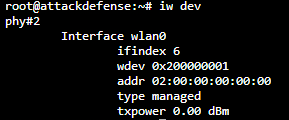
\includegraphics[scale=1]{img/interface_wlan0.png}
            \caption{Interfaces disponibles}
            \label{fig:step2}
        \end{figure}

        \begin{figure}[!h]
            \centering
            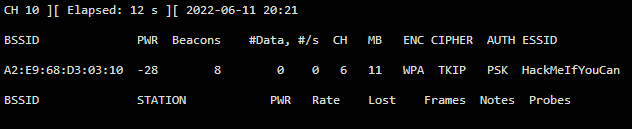
\includegraphics[scale=0.8]{img/airodump.png}
            \caption{Redes disponibles}
            \label{fig:step3}
        \end{figure}

        \clearpage
        \begin{figure}[!h]
            \centering
            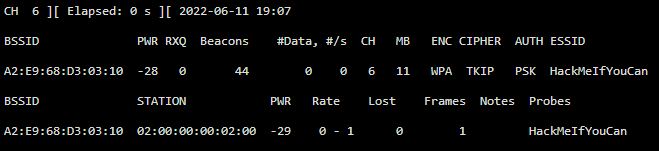
\includegraphics[scale=0.8]{img/-c6-wtest.png}
            \caption{Conexiones a la red}
            \label{fig:step4}
        \end{figure}

        \begin{figure}[!h]
            \centering
            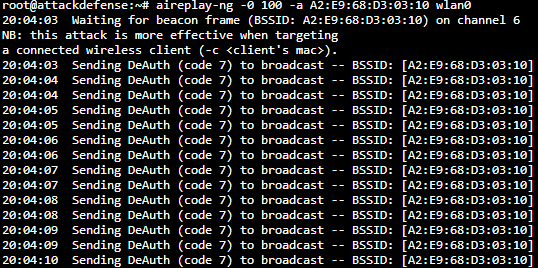
\includegraphics[scale=0.8]{img/aireplay.png}
            \caption{Envío de paquetes de de-autenticación}
            \label{fig:step5}
        \end{figure}

        \clearpage
        \begin{figure}[!h]
            \centering
            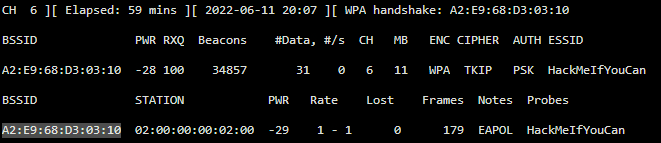
\includegraphics[scale=0.7]{img/handshake_captured.png}
            \caption{Captura del WPA Handshake}
            \label{fig:step6}
        \end{figure}

        \begin{figure}[!h]
            \centering
            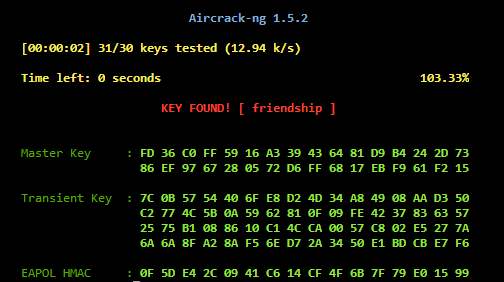
\includegraphics[scale=0.7]{img/flag.png}
            \caption{Clave encontrada}
            \label{fig:step7}
        \end{figure}

        \clearpage
        \begin{landscape}
            \begin{figure}[!h]
                \centering
                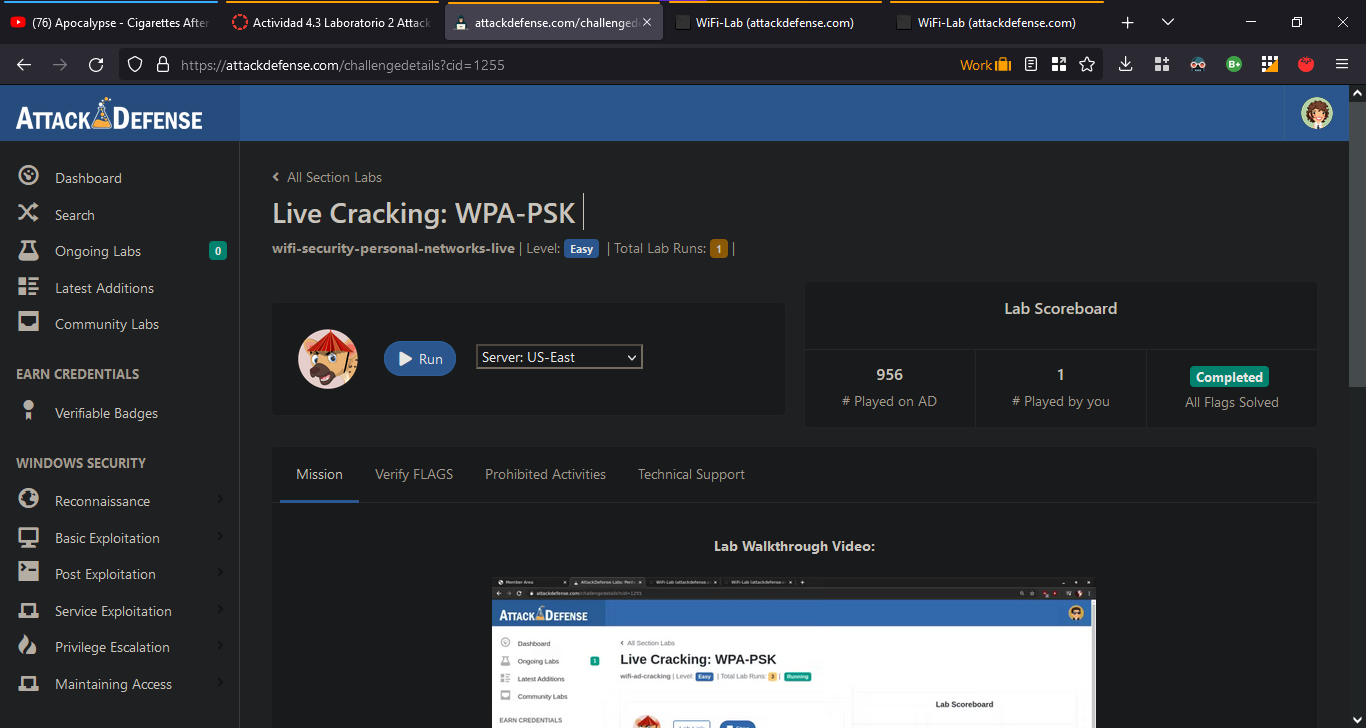
\includegraphics[scale=0.5]{img/wpa-breaking-after-evidence.png}
                \caption{Evidencia de finalización de actividad}
                \label{fig:wpa-after}
            \end{figure}
        \end{landscape}

\end{document}